\chapter{Algorithms, data structures, and formal reasoning}
\label{ch:algorithms}

\section{A motivating problem}
CivicQueue may store 100 appointments today and ten million historical records next year. A search that feels instant on a laptop can become unusable at scale. Choosing an algorithm and data structure is therefore a design decision about time, memory, correctness, and future change.

\learningobjectives{You should be able to use sets, relations, functions, sequences, trees, and graphs; explain invariants and induction; implement common data structures; analyse time and space asymptotically; and distinguish asymptotic reasoning from measured performance.}

\section{Sets, relations, and functions}
A set is a collection of distinct elements. If $A=\{1,2,3\}$, then $2\in A$ means 2 is a member. A relation $R$ between sets $A$ and $B$ is a set of ordered pairs from $A\times B$. A function $f:A\to B$ is a relation with exactly one output in $B$ for each input in $A$.

These ideas appear in systems. Let $U$ be users and $P$ be permissions. A relation \texttt{can\_access} \(\subseteq U\times P\) records grants. It may not be a function: one user can have several permissions, and several users can share one permission. Confusing a relation with a function causes bad data models and incorrect code.

\section{Data structures as representations}
An array provides indexed access. A stack supports last-in, first-out operations. A queue supports first-in, first-out operations. A hash table maps keys to buckets using a hash function. A tree represents hierarchy; a graph represents arbitrary relationships.

\begin{figure}[H]
\centering
\begin{tikzpicture}[every node/.style={font=\small}, cell/.style={draw, minimum width=12mm, minimum height=9mm, fill=pale}, arr/.style={-{Latex}, thick, blue}]
\node[cell] (a) at (0,0) {A};\node[cell,right=0pt of a] (b) {B};\node[cell,right=0pt of b] (c) {C};\node[cell,right=0pt of c] (d) {D};
\node[above=5mm of b] {array indices};
\node[below=12mm of a] (s1) {top};\node[below=12mm of b] (s2) {next};\node[below=12mm of c] (s3) {next};
\draw[arr] (s1)--(a);\draw[arr] (s2)--(b);\draw[arr] (s3)--(c);
\end{tikzpicture}
\caption{A sequence can support several abstract data types, but the operations and invariants differ.}
\label{fig:data-structures}
\end{figure}

An abstract data type specifies allowed operations and their meaning without fixing an implementation. A queue can be implemented by a list, a linked structure, or a concurrent service. The abstraction helps clients depend on behaviour rather than representation.

\section{Correctness through invariants}
An invariant is a proposition that is true before and after every operation that preserves the data structure. For a queue, an invariant might be that the front element is the oldest element not yet removed. To reason about a loop, identify:
\begin{enumerate}
\item the invariant before the first iteration;
\item why one iteration preserves it;
\item what the invariant implies when the loop stops.
\end{enumerate}
This is a practical form of proof. It can be applied to a cursor in a database query, a parser, or a simulation update.

\section{Induction and recursion}
Mathematical induction proves a statement for all natural numbers. First prove the base case. Then assume it holds for an arbitrary $n$ and prove it holds for $n+1$. Recursive programs use a related structure: a base case and a recursive case that reduces the problem to a smaller instance. A recursive function without a reachable base case does not terminate.

For the sum $1+2+\cdots+n$, define $S(0)=0$ and $S(n)=n+S(n-1)$. The recurrence makes the reasoning explicit. An iterative implementation may be preferable in Python when recursion depth is large.

\section{Searching and sorting}
Linear search checks elements one by one. If the target is equally likely to be anywhere, its average number of comparisons is approximately $(n+1)/2$ when it exists and $n$ when it does not. Binary search repeatedly halves a sorted search interval. Its logarithmic behaviour depends on the precondition that the data is sorted and that the index operation is efficient.

Sorting algorithms illustrate trade-offs. Insertion sort is simple and useful for small or nearly sorted inputs. Merge sort offers $O(n\log n)$ worst-case time and uses extra space. Quicksort is often fast in practice but can have $O(n^2)$ worst-case time unless the pivot strategy and input assumptions are controlled. A library implementation may be preferable because it has been engineered and tested across cases.

\section{Asymptotic notation}
We write $f(n)\in O(g(n))$ if there are constants $c>0$ and $n_0$ such that
\[
0\le f(n)\le c\,g(n) \quad \text{for every }n\ge n_0.
\]
The variable $n$ measures input size. The notation describes an eventual upper bound up to constant factors. It ignores constant costs, hardware, cache behaviour, interpreter overhead, and distribution of inputs. Therefore $O(n)$ is not automatically faster than $O(n\log n)$ for small $n$, and the label does not predict latency without a cost model.

Space complexity applies the same idea to additional memory. A streaming algorithm may use $O(1)$ extra space while taking $O(n)$ time. A hash table may offer expected $O(1)$ lookup under assumptions about hashing and load, while requiring $O(n)$ storage.

\begin{figure}[H]
\centering
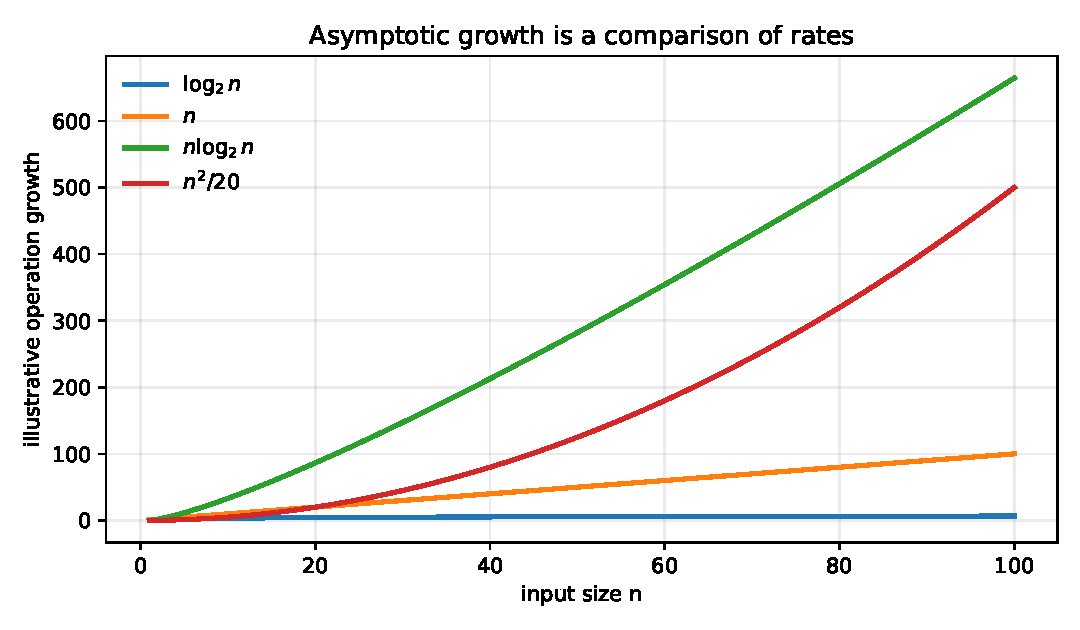
\includegraphics[width=0.78\linewidth]{figures/complexity-plot.pdf}
\caption{Illustrative growth curves generated by \texttt{figures/complexity\_plot.py}. The plot is a teaching aid, not a benchmark.}
\label{fig:complexity}
\end{figure}

\section{Graphs and networks}
A graph $G=(V,E)$ consists of vertices $V$ and edges $E$. Edges may be directed or undirected and may carry weights. In CivicQueue, a graph could represent dependencies among services, escalation paths, or relations among organisations. Breadth-first search explores by distance in an unweighted graph; Dijkstra's algorithm solves shortest paths when edge weights are non-negative. The representation and query determine which algorithm is appropriate.

\section{Measured performance}
Asymptotic analysis and measurement answer different questions. A benchmark should state hardware, software version, input generation, warm-up, repetitions, timing method, and variability. Avoid measuring a toy implementation and generalising to a production system. Profile before optimising; a theoretically elegant algorithm cannot compensate for a database query that returns unnecessary rows or a network call made inside a loop.

\section{Project application}
For any non-trivial feature, record the data structure, operation costs, input-size assumptions, and correctness invariant. When documenting the work, justify the choice in relation to the problem rather than listing Big-O labels. When presenting it, explain a failure case: an unsorted input to binary search, a hash collision, a disconnected graph, or an unexpectedly large recursion depth.

\section{Summary and key terms}
Formal structures clarify what data means. Algorithms are procedures with preconditions, operations, and correctness claims. Invariants and induction provide reusable reasoning tools. Asymptotic notation describes growth under explicit assumptions; measurement is still needed for engineering decisions.

\begin{keyterms}set; relation; function; sequence; abstract data type; array; stack; queue; hash table; tree; graph; invariant; induction; recursion; sorting; searching; asymptotic notation; scalability.\end{keyterms}

\section{Exercises and worked solutions}
\exercise{A list contains 1,000,000 user identifiers. When is a set a better representation than a list?}
\solution{If the main operation is membership testing and order is not required, a set usually offers expected constant-time membership rather than linear scanning. It uses additional memory and depends on hash behaviour. If stable ordering or duplicate values matter, another representation may be more suitable.}

\exercise{State the loop invariant for a linear search that has examined positions $0$ through $i-1$.}
\solution{The target is not present in positions $0$ through $i-1$, unless the algorithm has already returned. Initially the range is empty, so the invariant holds. Each iteration checks the next position and preserves the claim if the target is not found. When $i=n$, the invariant establishes that the target is absent.}

\exercise{Why is binary search not valid on an arbitrary list?}
\solution{Binary search discards half of the remaining range because sorted order guarantees that all values on one side are too small or too large. Without sorted order, discarding a side can discard the target. The algorithm's logarithmic bound depends on this precondition.}

\section{Further reading}
See \citet{cormen2022introduction} for algorithms and correctness, and \citet{knuth1997art} for a deeper historical treatment of representation and analysis.
